\documentclass[conference]{IEEEtran}
\usepackage{cite}
\usepackage{amsmath,amssymb}
\usepackage{graphicx}
\usepackage{booktabs}
\usepackage{multirow}
\usepackage{url}
\usepackage{xcolor}
\usepackage{tikz}
\usetikzlibrary{arrows.meta,positioning,fit,calc}

\newcommand{\ada}[1]{ADA~#1}

\begin{document}

\title{From LLM-Generated Buildings to Graph Agents:\\Wheelchair Accessibility Checking of IFC Models\\under the 2010 ADA Standards}

\author{\IEEEauthorblockN{\"Omer Can Atl\i}
\IEEEauthorblockA{Department of Computer Engineering\\
Gebze Technical University\\
Kocaeli, T\"urkiye}}

\maketitle

\begin{abstract}
Automated compliance checking of building information models is usually rule-based and therefore depends on
complete, consistently modelled data, while learning-based checkers lack labelled models to learn from. We present
a pipeline for wheelchair accessibility of single-storey buildings that (i) lets a large language model (LLM)
generate labelled buildings, which our code writes to IFC and a rule engine verifies and labels, (ii) distils this
generator into a 7B student model, (iii) converts each IFC file into a room--door graph on which three graph neural
network (GNN) agents assess the doors, the rooms and the reachability from the entrance, and (iv) combines their
findings in a main agent that returns a building-level verdict and the violated ADA rule. From 231 teacher
buildings, a LoRA-tuned Qwen2.5-7B student produced 2,013 valid buildings (81\% of its attempts, against 4\% for the
untuned model). On 336 unseen buildings the system reaches a building-level macro F1 of 0.938 with a main agent that
traces the path over the agents' findings; a fine-tuned 7B LLM main agent reaches 0.921 (difference not
significant), whereas the untuned 7B model does not exceed 0.57. Training the agents with randomly deleted values
improves them on complete data and keeps the system usable when values are missing: with 30\% of the values
deleted it misses 3 of 225 inaccessible buildings, against 72 for a rule engine that skips unknown values. A first
test on 20 public IFC models shows what does not yet transfer: real files carry no accessibility properties, and
estimated door widths depend on the authoring tool's conventions.
\end{abstract}

\begin{IEEEkeywords}
Building information modeling, IFC, accessibility, ADA, automated code checking, graph neural networks,
large language models, knowledge distillation.
\end{IEEEkeywords}

\section{Introduction}

Accessibility regulations such as the 2010 ADA Standards for Accessible Design~\cite{ada2010} set measurable
requirements for a wheelchair user: the clear width of a door, the clear floor space in front of it, the diameter
of a turning space. Checking them on a building information model (BIM) exchanged as IFC~\cite{iso16739} moves the
design review to a stage where changes are still cheap.

Rule-based checkers~\cite{eastman2009,solihin2015} are precise when the model is complete and modelled as the
rules expect, but they are brittle otherwise: a value that is not in the file can only be skipped or assumed to
fail. Learning-based checkers~\cite{bloch2023aei,bloch2023icccbe} can tolerate imperfect data, yet they need
labelled building models, which are scarce. Large language models can produce building models~\cite{du2024text2bim}
and compliance-checking code~\cite{fuchs2026}, but the large models involved are costly to run at scale and were not
used to create training data for a checker.

This paper connects these lines for one concrete question: \emph{is this building accessible to a wheelchair user,
and if not, which element violates which ADA rule?} We study single-storey buildings and six ADA requirements on
doors, rooms and routes. Our contributions are:
\begin{enumerate}
\item a generation loop in which code fixes the layout and the values near each limit, an LLM describes the
building, our code writes the IFC file, and a rule engine verifies and labels it; the loop is distilled into a 7B
student that produces nearly nine times the teacher's data;
\item three GNN agents on a room--door graph read from the IFC file, including a reachability agent on a
\emph{transit graph} that represents whether a room can be crossed without turning;
\item a comparison of main agents (path tracing, zero-/few-shot LLMs, a fine-tuned 7B LLM) that shows when an LLM
judge adds value over the agents;
\item an experiment with missing values and a first test on public IFC models, which show what transfers to real
files and what does not.
\end{enumerate}

\section{Related Work}

\textbf{Rule-based checking.} Eastman et al.~\cite{eastman2009} describe the structure of rule-checking systems
(rule interpretation, building model preparation, rule execution, reporting); Solihin and
Eastman~\cite{solihin2015} classify rules by the complexity of the model data they need. Both stress that the
model must carry the data the rules expect, which real exports often do not.

\textbf{Learning-based checking.} Bloch et al.~\cite{bloch2023aei} propose graph-based learning as an alternative
to hard-coded rule sets and illustrate it with accessibility requirements in residential houses. In a companion
study~\cite{bloch2023icccbe} a GNN trained on synthetic data reaches 86\% accuracy on its test set and 82\% in the
accessibility check of a real model. We share the graph view and the synthetic training data, but generate the data
with an LLM, split the check into specialised agents, and add a main agent that names the violated rule.

\textbf{LLMs for BIM.} Text2BIM~\cite{du2024text2bim} lets several LLM agents generate building models through the
API of an authoring tool, exports them to IFC and feeds the issues of a rule-based model checker back to the
agents; its rules cover geometry, clashes and information, not accessibility. Fuchs et al.~\cite{fuchs2026} let an
LLM agent write reusable compliance-checking functions against IFC models and report that geometric reasoning that
needs auxiliary constructions remains difficult. We use the LLM neither to design nor to write the checker: it
creates labelled training data, and it judges the agents' findings.

\textbf{Distillation and LLM judges.} Knowledge distillation~\cite{hinton2015} transfers the behaviour of a large
model to a small one; LLM-generated instruction data~\cite{wang2023selfinstruct} and parameter-efficient
fine-tuning~\cite{hu2022lora,dettmers2023qlora} make this practical for LLMs. Using an LLM to combine and judge
other outputs follows the LLM-as-a-judge setting~\cite{zheng2023judge}.

\section{Problem and Rules}

The scope is one storey and a wheelchair user. Table~\ref{tab:rules} lists the six requirements. The maneuvering
clearance of \ada{404.2.4} is simplified to a front approach: the clear depth in front of the door must be at least
1525\,mm on the pull side and 1220\,mm on the push side.

\begin{table}[t]
\caption{ADA requirements checked and the agent responsible}
\label{tab:rules}
\centering
\resizebox{\columnwidth}{!}{%
\begin{tabular}{@{}llll@{}}
\toprule
ADA & Requirement & Limit (mm) & Agent \\
\midrule
404.2.3 & door clear width & $\geq 815$ & door \\
404.2.5 & threshold height & $\leq 13$ & door \\
404.2.7 & door hardware height & 865--1220 & door \\
404.2.4 & maneuvering clearance & pull $\geq 1525$, push $\geq 1220$ & door \\
304.3.1 & turning space diameter & $\geq 1525$ & room \\
403.5.1 & straight passage width & $\geq 915$ & route \\
\bottomrule
\end{tabular}}
\end{table}

The verdict follows four rules. (1) A door that fails any of its rules cannot be passed. (2) A room whose turning
space fails can still be entered (a warning), but it can only be crossed in a straight line: the doors used to enter
and to leave it must lie on \emph{opposite} walls and the room must be at least 915\,mm wide across the way
(\ada{403.5.1}); doors on \emph{adjacent} walls require a 90$^\circ$ turn, so the rooms behind are unreachable. The
wall of a door is taken from the IFC geometry; if it is unknown, a turn is assumed. (3) A rule whose value is
neither in the file nor estimable is reported as \emph{not checked} and does not fail the element. (4) The building
is \emph{accessible} if every room can be reached from the entrance; the violated rules are those on the way to an
unreachable room, and failures that block no room (e.g., the last room cannot be turned in) are warnings.

\section{Method}

Fig.~\ref{fig:pipeline} shows the pipeline. Rooms are named R1, R2,\,\dots{} and doors D1, D2,\,\dots{}; the
rule engine is used only to verify and label generated buildings, never inside the check.

\begin{figure*}[t]
\centering
\resizebox{\textwidth}{!}{%
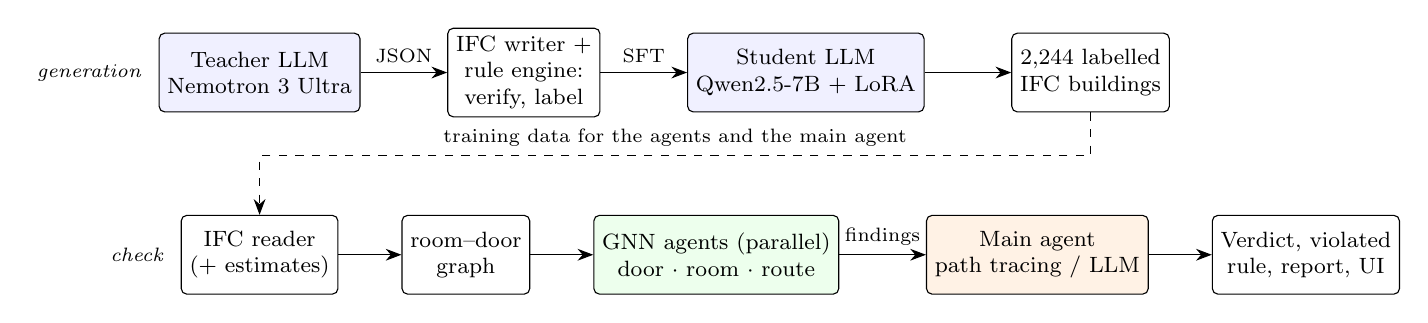
\begin{tikzpicture}[
  box/.style={draw, rounded corners=2pt, align=center, font=\footnotesize, minimum height=10mm, inner sep=3pt, fill=#1},
  box/.default=white, >={Stealth[length=2mm]}, node distance=11mm]
\node[box=blue!6] (t) {Teacher LLM\\Nemotron 3 Ultra};
\node[box, right=of t] (v) {IFC writer +\\rule engine:\\verify, label};
\node[box=blue!6, right=of v] (s) {Student LLM\\Qwen2.5-7B + LoRA};
\node[box, right=of s] (d) {2,244 labelled\\IFC buildings};
\node[box, below=13mm of t] (r) {IFC reader\\(+ estimates)};
\node[box, right=8mm of r] (g) {room--door\\graph};
\node[box=green!7, right=8mm of g] (a) {GNN agents (parallel)\\door $\cdot$ room $\cdot$ route};
\node[box=orange!10, right=of a] (m) {Main agent\\path tracing / LLM};
\node[box, right=8mm of m] (o) {Verdict, violated\\rule, report, UI};
\draw[->] (t) -- node[above, font=\scriptsize]{JSON} (v);
\draw[->] (v) -- node[above, font=\scriptsize]{SFT} (s);
\draw[->] (s) -- (d);
\draw[->] (r) -- (g); \draw[->] (g) -- (a); \draw[->] (a) -- node[above, font=\scriptsize]{findings} (m); \draw[->] (m) -- (o);
\draw[->, dashed] (d.south) -- ++(0,-5.5mm) -| (r.north)
  node[pos=0.25, above, font=\scriptsize]{training data for the agents and the main agent};
\node[font=\scriptsize\itshape, anchor=east] at ($(t.west)+(-1mm,0)$) {generation};
\node[font=\scriptsize\itshape, anchor=east] at ($(r.west)+(-1mm,0)$) {check};
\end{tikzpicture}}
\caption{Pipeline. Top: an LLM describes labelled buildings as JSON, our code writes and verifies the IFC file, and
the teacher's verified answers fine-tune a 7B student that generates most of the data. Bottom: an IFC file is read
into a graph, three GNN agents assess it in parallel, and a main agent gives the building-level verdict.}
\label{fig:pipeline}
\end{figure*}

\subsection{Building representation and IFC}

The LLM describes a building as JSON: rooms with position, size and turning-space diameter; doors with the two
spaces they connect (or \textsc{exterior}), their position on a wall and the five door values of
Table~\ref{tab:rules}. The LLM never writes IFC. Our writer (IfcOpenShell~\cite{ifcopenshell}) creates IFC4 or
IFC2X3 files with walls, spaces, doors in wall openings, space boundaries and a property set
\texttt{ADA\_Accessibility}; our reader recovers the same JSON from the property sets and the placement geometry,
including the wall each door lies on. Every labelled building is read back from its IFC file before it reaches an
agent, so the agents see what they would see at run time. Fields that state the answer (e.g.,
\texttt{HandicapAccessible}) are never given to an agent.

\subsection{Teacher generation and verification}

Each building is a separate request: a fixed system prompt and a scenario prompt. Nine scenarios define the
target verdict and its cause: all compliant; D2 fails one of its four rules (four scenarios); the entrance door D1
fails; R1 cannot turn and D1, D2 lie on adjacent walls (not accessible); R1 cannot turn but can be crossed in a
straight line (accessible, warning); R2 cannot turn (accessible, warning).

Because every request is independent, the model does not see its earlier buildings and returns to the same values:
in an early prompt version, 27 of 36 doors had a 1000\,mm hardware height and R2 always lay east of R1. The final
prompt therefore lets \emph{code} fix what must vary: the direction of R2, the walls of D1 and D2 (consistent with
the scenario's adjacent or opposite condition), approximate room sizes, the hardware type, and the exact failing
value, half of them 1--30\,mm beyond the limit; half of the prompts also ask for a compliant value close to a
limit. All limits come from one configuration file.

A building is kept only if its JSON is complete and plausible (doors 600--1200\,mm, rooms 2500--6000\,mm,
turning space not larger than the room's shorter side, every door on a wall), the maneuvering clearance on each side
does not exceed the depth of the room on that side, the doors lie on the walls the prompt asked for, the rule
engine's verdict and violated rules equal the scenario's, and the model's own stated verdict equals the rule
engine's. The rule engine then writes the labels: the verdict, the failing rules per door, the turning result per
room and the reachability per room, i.e., the targets of the main agent and of the three GNN agents.
The teacher is \texttt{nemotron-3-ultra-550b-a55b}~\cite{nemotron}, which returns a reasoning trace.

\subsection{Student distillation}

The teacher's verified answers (reasoning trace and JSON) fine-tune Qwen2.5-7B-Instruct~\cite{qwen2025} with
LoRA~\cite{hu2022lora} (rank 16, $\alpha=32$, all linear layers). The loss covers only the answer; examples longer
than 10,240 tokens are dropped rather than truncated, since a cut answer would teach the student to stop inside the
JSON. Training took 20 minutes (3 epochs) on one A100 GPU in 16-bit precision. The student is served with
vLLM~\cite{kwon2023vllm} and goes through the same prompts and the same verification as the teacher.

\subsection{Graph and agents}

Rooms are nodes with width, length and turning-space diameter, three missing-value flags and an exterior flag
(7 features); doors are edges with their five values, five missing-value flags and the wall the door lies on in
each of the two rooms (one-hot S/N/W/E/unknown; 20 features). Values are standardised with the training split's
mean and standard deviation after clamping to its range, so that values outside the training range (real files) are
not extrapolated; a missing value becomes 0 with its flag set. All models are built with PyTorch
Geometric~\cite{fey2019pyg}.

The \emph{door agent} (two GINE layers~\cite{xu2019gin,hu2020gine}) predicts four logits per door, one per door
rule. The \emph{room agent} (four GINE layers) predicts whether a room's turning space fails. The \emph{route agent}
predicts whether each room is reachable from the entrance. Its difficulty is geometric: whether R2 can be reached
through a room that cannot turn depends on the walls of \emph{two} doors of that room at once, which a message along
one door edge does not see. The route agent therefore derives a directed transit graph (Fig.~\ref{fig:transit}):
a transit node is ``entering room $r$ through door $d$'', and a transit edge is ``crossing $r$ from door $d_1$ to door
$d_2$'', carrying the walls of both doors and the features of $r$. Messages are aggregated with a maximum, as a
single blocked door suffices to block a path~\cite{gilmer2017}, and a room's logit is the maximum over the transit
nodes entering it. All agents use a weighted binary cross-entropy (positive weight at most 20), early stopping on
the validation F1, three seeds, and a decision threshold per output chosen on the validation split.

\begin{figure}[t]
\centering
\resizebox{\columnwidth}{!}{%
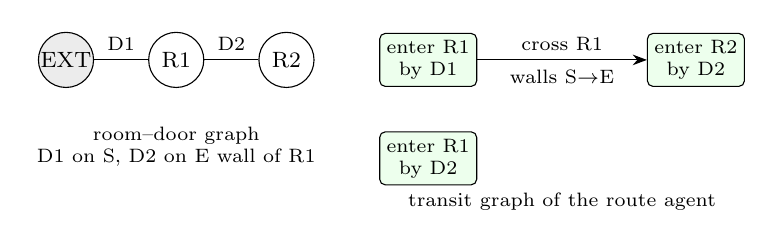
\begin{tikzpicture}[
  room/.style={circle, draw, minimum size=7mm, font=\footnotesize, inner sep=0pt},
  tn/.style={draw, rounded corners=2pt, font=\scriptsize, fill=green!7, inner sep=2.5pt, align=center},
  >={Stealth[length=1.8mm]}]
\node[room, fill=gray!15] (e) at (0,2) {EXT};
\node[room] (r1) at (1.4,2) {R1};
\node[room] (r2) at (2.8,2) {R2};
\draw (e) -- node[above, font=\scriptsize]{D1} (r1);
\draw (r1) -- node[above, font=\scriptsize]{D2} (r2);
\node[font=\scriptsize, align=center] at (1.4,0.9) {room--door graph\\D1 on S, D2 on E wall of R1};
\node[tn] (a) at (4.6,2) {enter R1\\by D1};
\node[tn] (c) at (8.0,2) {enter R2\\by D2};
\node[tn] (b) at (4.6,0.75) {enter R1\\by D2};
\draw[->] (a) -- node[above, font=\scriptsize]{cross R1} node[below, font=\scriptsize]{walls S$\to$E} (c);
\node[font=\scriptsize] at (6.3,0.2) {transit graph of the route agent};
\end{tikzpicture}}
\caption{The route agent's transit graph. A transit edge carries the walls of the entry and exit doors of the room
it crosses, so ``R1 cannot turn and D1, D2 are on adjacent walls'' is visible on a single edge.}
\label{fig:transit}
\end{figure}

\textbf{Training with missing values.} Real files lack most of the values the rules need. Optionally, every
measured value of a training batch is deleted with probability $p=0.2$ (value 0, flag 1; a door identically in both
edge directions; room width and length are geometry and are never deleted), while the targets remain those of the
complete building. The agent then has to infer a missing value's rule from the rest of the building.

\subsection{Main agent}

The main agent receives the agents' findings as JSON: per door the four failure probabilities, its values and its
walls; per room the turning and reachability probabilities and its values; and which values were estimated or not
checked. It returns the verdict, the violated rules, warnings and an explanation. We compare:

\emph{Path tracing (no LLM).} A breadth-first search from \textsc{exterior} passes a door unless the door agent
predicts a failing rule, and crosses a room the room agent marks as unable to turn only through doors on opposite
walls of a room at least 915\,mm wide. It uses the agents' predictions and the door walls, not the door limits; the
route agent serves as a second opinion and its disagreements are reported as warnings.

\emph{Route agent.} A room is reachable if the route agent says so (the original design).

\emph{LLM judges.} The same findings and a system prompt that explains the rules and asks the model to trace the
path itself~\cite{zheng2023judge}: GPT-OSS-20B~\cite{gptoss2025} and Qwen2.5-7B-Instruct, zero-shot and with four
hand-made worked examples; and Qwen2.5-7B fine-tuned with LoRA on the agents' findings for the 1,908 training and
validation buildings, with the labels as targets and an explanation that traces the path written \emph{before}
the verdict. An answer that is not valid JSON with known labels and rules counts as wrong.

\subsection{Real files}

Real IFC exports carry no accessibility property set. The reader estimates what standard IFC data allows: the clear
width as $(\text{OverallWidth} - 2\cdot\text{lining})\cdot\text{leaf share} - \text{open leaf thickness}$, the
maneuvering clearance on each side from the depth of the adjacent room (the pull side, which is unknown, gets the
shallower one), and the turning space as the shorter side of the empty room (an upper bound). Hardware height has no
IFC field and is never estimated. Estimated values are marked in the report; what cannot be estimated is
\emph{not checked}. Since the scope is one storey, the reader checks the lowest storey that has spaces and an
external door (\texttt{Pset\_DoorCommon.IsExternal}), or else the storey nearest to elevation 0.

\section{Experimental Setup}

The data set holds 2,244 buildings: 231 from the teacher and 2,013 from the student, all with two rooms. It is split
by building, 70/15/15\% with a fixed seed, into 1,571 training, 337 validation and 336 test buildings; the test split
contains 225 inaccessible and 111 accessible buildings, and no test building is used for any training. Agents are
scored by the F1 of their failing class (door fails, room cannot turn, room unreachable), with a target of 0.85. The
building verdict is scored by macro F1 over the two classes, with a target of 0.90; always predicting the majority
class gives 0.40. Violated rules are scored as precision, recall and F1 over (element, rule) pairs and as the rate of
exact matches. Paired comparisons on the same buildings use the exact McNemar test~\cite{mcnemar1947}. GNNs were
trained on a CPU; LLMs were trained and served on one A100 GPU; GPT-OSS-20B was queried through a hosted API.

\section{Results}

\subsection{E1: Generation and distillation}

\begin{table}[t]
\caption{E1: Valid buildings per generator}
\label{tab:e1}
\centering
\resizebox{\columnwidth}{!}{%
\begin{tabular}{@{}lrrr@{}}
\toprule
Generator & Valid / attempts & Rate & Tokens / answer \\
\midrule
Teacher (Nemotron 3 Ultra) & 231 / 231 & 100\% & 4,271 \\
Student (Qwen2.5-7B + LoRA) & 2,013 / 2,493 & 81\% & 4,272 \\
Untuned Qwen2.5-7B & 2 / 50 & 4\% & 413 \\
\bottomrule
\end{tabular}}
\end{table}

Table~\ref{tab:e1} shows that distillation transfers the task: the untuned 7B model failed mainly by placing doors on
walls other than those requested (37 of its 48 rejections), whereas the student passes 81\% of the checks, at 63\,s
per request on one GPU (16 parallel requests) against 93\,s for the teacher through an API (4 parallel). The student's rejections were doors on a wrong
wall (246), a maneuvering clearance deeper than the room (97), a stated verdict that contradicts the rule engine
(93) and invalid JSON (59, of which 48 hit the 10,000-token limit). The student also copied the teacher's answer
length and its uniformity: 3,432 of 4,026 doors have a 1000\,mm hardware height, the value no prompt fixes. Values
near the limits, which the prompts fix, are covered about ten times more often than in the teacher's data.

\subsection{E2: Agents}

\begin{table}[t]
\caption{E2: Agent F1 of the failing class on the test split (mean $\pm$ std over 3 seeds)}
\label{tab:e2}
\centering
\resizebox{\columnwidth}{!}{%
\begin{tabular}{@{}lcc@{}}
\toprule
Agent & complete training data & values deleted ($p=0.2$) \\
\midrule
Door (any rule) & 0.901 $\pm$ 0.004 & \textbf{0.926} $\pm$ 0.006 \\
\quad 404.2.3 width & 0.954 & 0.953 \\
\quad 404.2.5 threshold & 0.993 & 1.000 \\
\quad 404.2.7 hardware & 0.894 & 0.936 \\
\quad 404.2.4 maneuvering & 0.728 & 0.796 \\
Room (turning space) & 0.925 $\pm$ 0.005 & \textbf{0.960} $\pm$ 0.016 \\
Route, max-aggregation MPNN & 0.845 $\pm$ 0.016 & -- \\
Route, transit graph & \textbf{0.893} $\pm$ 0.010 & 0.879 $\pm$ 0.008 \\
\bottomrule
\end{tabular}}
\end{table}

All three agents exceed the 0.85 target (Table~\ref{tab:e2}). With the 231 teacher buildings alone the door and
room agents memorised the training set (training F1 1.00, test 0.6--0.7, door 0.71 and room 0.76 after input
standardisation); the student's data closed most of the gap, and training with deleted values part of the rest.
The weakest rule remains \ada{404.2.4}: its values spread over 700--6000\,mm, and half of the failing ones lie only
1--30\,mm beyond the limit, which a decision tree on the same features finds exactly (F1 1.00 for doors and rooms)
but a neural network only approximates. For the route agent, message passing on the room--door graph (GINE 0.827,
max-aggregation MPNN 0.845) failed on geometry: in the scenario where R1 cannot turn but can be crossed straight,
28 of 40 test buildings were wrong. On the transit graph only 4 of 40 were wrong.

\subsection{E3: Main agents}

\begin{table}[t]
\caption{E3: Main agents on the 336 test buildings. Verdict macro F1; violated rules F1 and exact match}
\label{tab:e3}
\centering
\setlength{\tabcolsep}{4pt}
\begin{tabular}{@{}llccc@{}}
\toprule
Agents & Main agent & Verdict F1 & Rules F1 & Exact \\
\midrule
\multirow{6}{*}{\shortstack[l]{complete\\training}}
 & Route agent & 0.877 & -- & -- \\
 & Path tracing & 0.893 & 0.884 & 0.869 \\
 & GPT-OSS-20B, zero-shot & 0.899 & 0.896 & 0.881 \\
 & Qwen-7B, zero-shot & 0.569 & 0.595 & 0.533 \\
 & Qwen-7B, few-shot & 0.566 & 0.713 & 0.604 \\
 & Qwen-7B, fine-tuned & 0.916 & 0.911 & 0.902 \\
\midrule
\multirow{3}{*}{\shortstack[l]{values\\deleted}}
 & Route agent & 0.842 & -- & -- \\
 & Path tracing & \textbf{0.938} & 0.917 & 0.917 \\
 & Qwen-7B, fine-tuned & 0.921 & 0.923 & 0.914 \\
\midrule
Oracle & Path tracing & 1.000 & 1.000 & 1.000 \\
\bottomrule
\end{tabular}
\end{table}

Table~\ref{tab:e3} compares the main agents on identical findings. With perfect (oracle) agents, path tracing
reproduces every label, so all remaining errors come from the agents. Tracing the path over the door and room agents
beats asking the route agent directly in both settings. The untuned 7B LLM answered with valid JSON every time but
declared most accessible buildings inaccessible (F1 of the accessible class 0.31): it reported the failing values
correctly but did not decide whether they block a room, e.g., a room that cannot turn but is the last one; four
worked examples did not change this. GPT-OSS-20B, a reasoning model, matches path tracing (36 of its first answers
failed on the hosted API, 35 of them by time-out, and were requested again with the same findings).

Fine-tuning the 7B judge changes the picture. With the agents trained on complete data it reached 0.916 and was
significantly better than path tracing (8 buildings only it got right, 1 only path tracing, $p=0.039$): in 7 of the 8
buildings an agent had erred on a value a few millimetres from a limit, and the judge compared the raw value with
the limit it had learned from the labels. With the agents trained on deleted values, which make far fewer such
errors, path tracing reaches 0.938 and the fine-tuned judge 0.921 (3 vs.\ 8 buildings, $p=0.227$, not significant).
The judge's explanations are fluent but not always correct: among its errors are ``clear width 824\,mm $<$ 815\,mm'',
a room at exactly 1525\,mm called unable to turn, and an unreachable room asserted without any blocking element.

\subsection{E4: Missing values}

On the test split, a fraction of the measured values was deleted at random after reading the IFC file (three
deletion seeds, the same deletions for every system); the truth remains the label of the complete building.

\begin{table}[t]
\caption{E4: Verdict macro F1 with deleted values (mean of 3 seeds); in parentheses: missed inaccessible buildings
/ false alarms, out of 225 / 111}
\label{tab:e4}
\centering
\setlength{\tabcolsep}{3pt}
\resizebox{\columnwidth}{!}{%
\begin{tabular}{@{}lccc@{}}
\toprule
System & 10\% & 20\% & 30\% \\
\midrule
Rule engine, skip unknown & 0.925 (23/0) & 0.854 (47/0) & 0.782 (72/0) \\
Rule engine, unknown fails & 0.661 (0/77) & 0.494 (0/101) & 0.423 (0/109) \\
GNN (complete), skip & 0.832 (34/18) & 0.771 (53/19) & 0.724 (79/12) \\
GNN (complete), infer & 0.849 (26/19) & 0.795 (42/21) & 0.742 (68/16) \\
GNN (deleted), skip & 0.870 (27/13) & 0.799 (50/14) & 0.731 (76/13) \\
GNN (deleted), infer & 0.858 (3/36) & 0.802 (4/48) & 0.756 (3/58) \\
\bottomrule
\end{tabular}}
\end{table}

Table~\ref{tab:e4} must be read with one caveat: the rule engine wrote the labels, so on complete data it is correct
by construction (F1 1.000, against 0.893 and 0.938 for the two GNN systems). With missing values its two policies
sit at the extremes: skipping unknown values misses up to 72 inaccessible buildings, and treating them as failures
raises up to 109 false alarms. The GNN trained with deleted values, when its guess for a missing value is used
(\emph{infer}), misses 3--4 buildings at every level with about half the false alarms of the conservative rule
policy. Among the systems that do not miss inaccessible buildings it is far better (0.756 against 0.423 at 30\%), but
on macro F1 the skipping rule engine stays ahead. The guesses carry information: for missing values at 30\%, the
agent flagged 80 of 100 truly failing turning spaces but 31\% of the compliant ones (404.2.5: 44 of 46 vs.\ 37\%).
Part of this information may come from the structure of the synthetic data (e.g., the failing door is usually D2),
which would not transfer to real buildings; we have not separated the two.

\subsection{E5: Public IFC models}

We ran the check on the architectural models of 20 projects of the public ifc-bench collection~\cite{ifcbench}
(residential, office, hotel, clinic and hospital; ArchiCAD, Revit and other exporters; 456\,MB). All 20 files were
read (about 6\,s per file); two contain no \texttt{IfcSpace} and cannot be checked by a method built on spaces. The
selected storey is plausible for 16 of the remaining 18 files; in one file the elevations refer to sea level and no
door is marked external, so a basement was chosen. Fig.~\ref{fig:real} shows the result for a two-storey house.

All 18 checked buildings were judged inaccessible, almost always because of \ada{404.2.3} on an \emph{estimated}
door width, and this verdict cannot be trusted yet. \texttt{OverallWidth} means different things in different
exports: for a Revit~2011 door of type ``0915\,x\,2134\,mm'' it is the leaf itself (915\,mm), so subtracting a frame
gives 775\,mm and a probable false failure; for a Revit~2024 door of type ``900\,x\,2400\,mm'' it includes the frame
(1000\,mm) and the estimate of 860\,mm is reasonable; for pocket doors or curtain-wall doors it is meaningless. The
agents agreed with the rule engine on every file, because both decide on the same estimated values. Real models
have no ground truth here; a hand-checked sample is needed before any accuracy can be claimed.

\begin{figure}[t]
\centering
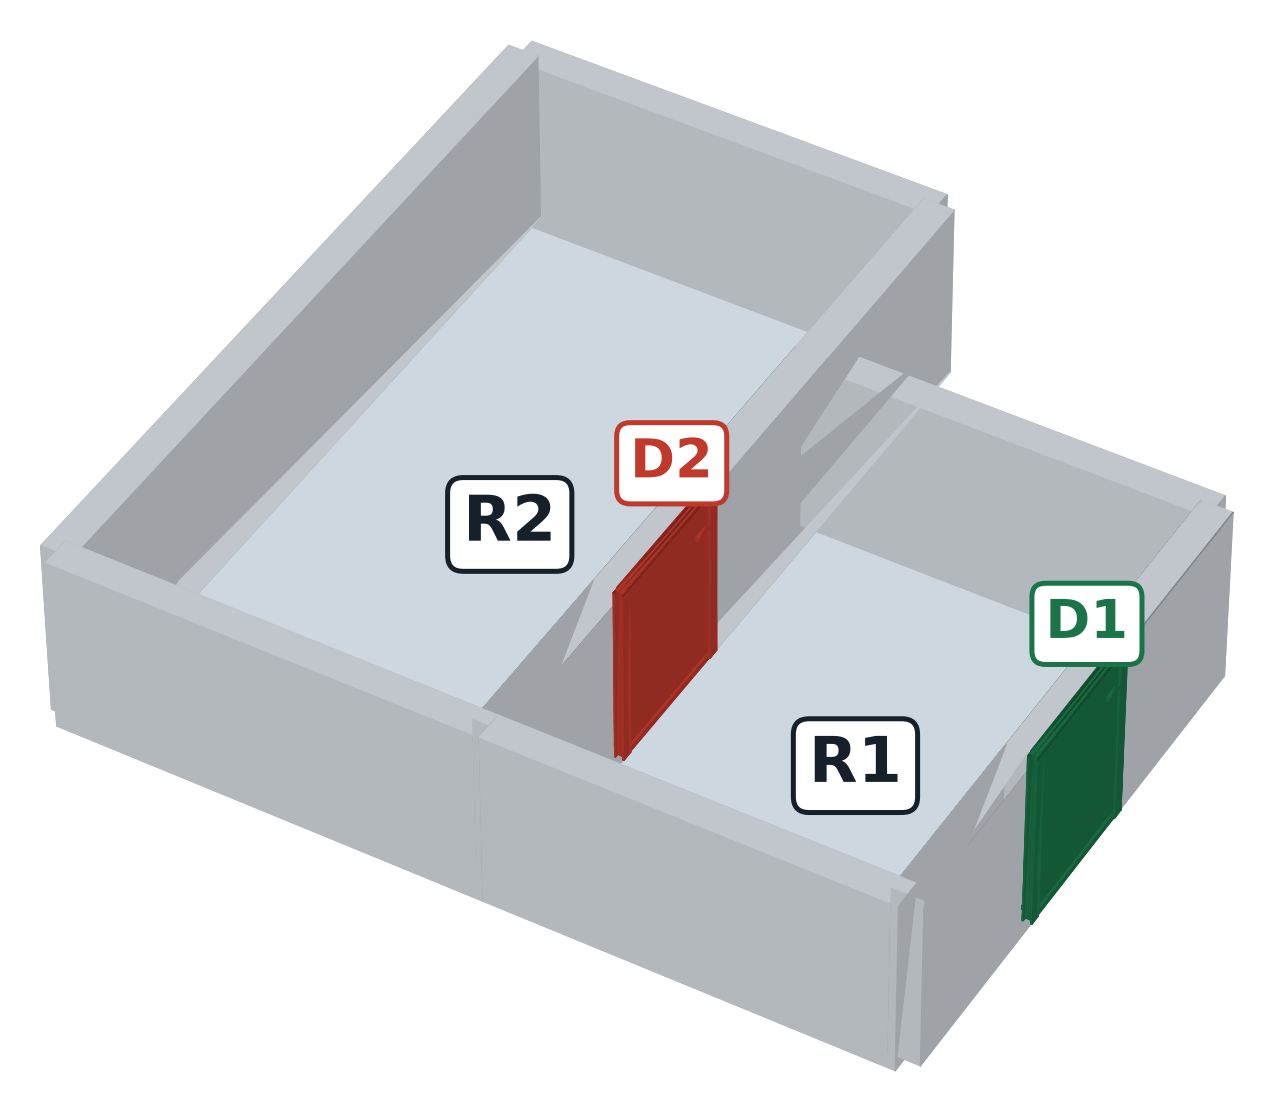
\includegraphics[width=0.48\columnwidth]{figures/synthetic_building.png}\hfill
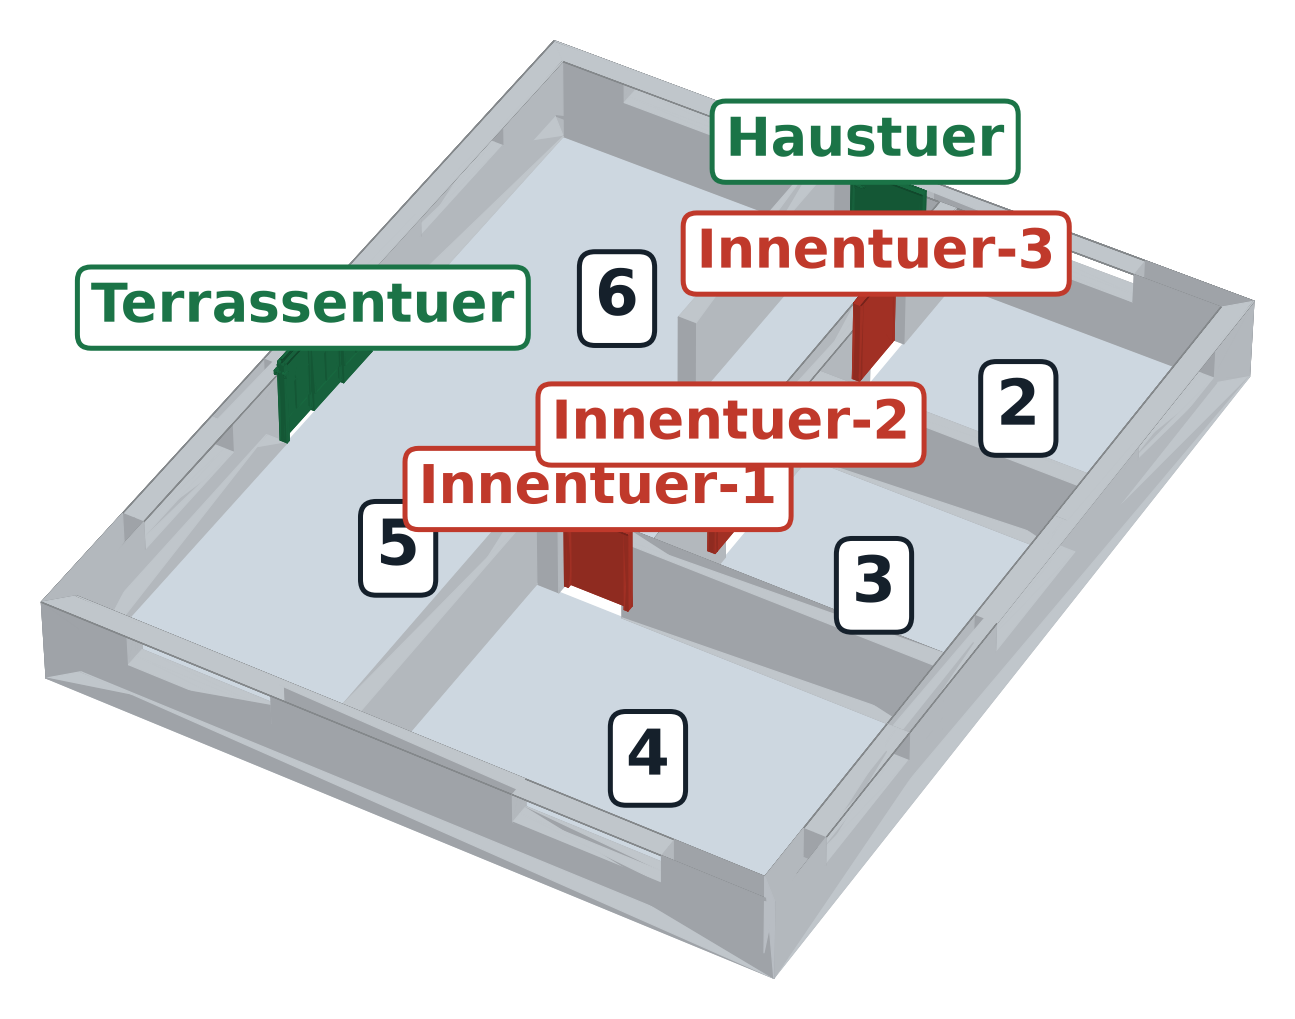
\includegraphics[width=0.48\columnwidth]{figures/fzk_house.png}
\caption{Left: a synthetic test building; D2 fails \ada{404.2.4} (push-side clearance 1196\,mm $<$ 1220\,mm), so R2
is unreachable. Right: the ground floor of a public two-storey model~\cite{ifcbench}; three inner doors fail on an
estimated clear width of 745\,mm (overall width 885\,mm). Failing doors are red.}
\label{fig:real}
\end{figure}

\section{Discussion}

\textbf{Where the learned system helps.} On complete synthetic data a rule engine is perfect by construction, and a
decision tree learns the door and room limits exactly. The case for learning lies in incomplete data, where the
agents trained with deleted values avoid both failure modes of fixed rules, and in the interface: the agents'
findings can be combined, questioned and explained. Deleting values during training also acted as a regulariser and
improved the agents on complete data, most for the rules whose failing values lie closest to the limit.

\textbf{When an LLM judge adds value.} An untuned 7B LLM cannot trace whether a failure blocks a room, even with
worked examples, while a 20B reasoning model can. A fine-tuned 7B judge adds value only while the agents make errors
it can correct from the raw values; with better agents the rule-based path tracing is as good and always
consistent with its explanation. LLM explanations should therefore not be shown without checking them against the
findings.

\textbf{Generating data with LLMs.} Fixing layout and near-limit values in code, verifying every building and
labelling it with a rule engine made LLM-generated buildings usable as training data, and a 7B student reproduced
the teacher's validity at lower cost. What the prompts did not fix, the models did not vary.

\section{Limitations and Future Work}

The buildings are synthetic, single-storey and have two rooms; corridors and larger layouts are untested. The labels
come from our own rule engine, so the agents learn our interpretation of the rules, which (adjacent walls require a
turn, the simplified \ada{404.2.4}, maneuvering clearance bounded by room depth) was not reviewed by architects. The
LLM results rest on single training runs. On real files the verdicts are unvalidated, door widths need an interval
estimate that reports ``not checked'' when the estimate spans the limit, and missing fields are systematic (no file
has a hardware height) rather than random as in E4. Next steps are a hand-labelled sample of real models, larger
buildings, systematic missing fields, and the fine-tuned judge under missing values.

\section{Conclusion}

An LLM can supply the labelled IFC buildings that a learning-based accessibility checker needs, provided that code
fixes what must vary and a rule engine verifies every building, and a 7B student can take over the generation.
Three GNN agents, including a reachability agent on a transit graph, and a main agent that traces the path over their
findings reach a building-level macro F1 of 0.938 on unseen buildings and remain usable when values are missing.
Whether this holds for real buildings depends on data that real files do not yet carry.

\bibliographystyle{IEEEtran}
\bibliography{references}

\end{document}
